\documentclass[a4paper, 10pt,onecolumn]{scrartcl}

%Standardpakete Deutsch
\usepackage[ngerman]{babel}
\usepackage[T1]{fontenc}
\usepackage[utf8]{inputenc}

%Extras
\usepackage{multirow}
\usepackage{natbib}
\usepackage{graphicx}
\usepackage{amsmath, amssymb}
\usepackage{graphicx}
\usepackage{grffile} %einfacheres einbinden von Dateipfaden
\usepackage{xpatch} %more space between title and subtitle
\usepackage{mathtools}
\usepackage{booktabs}
\newcommand{\changefont}[3]{
\fontfamily{#1} \fontseries{#2} \fontshape{#3} \selectfont}

\newlength{\myspace}
\setlength{\myspace}{2em}

\makeatletter
\xpatchcmd{\@maketitle}{\vskip.5em}{\vskip\myspace}{}{}
\makeatother

%\changefont{ptm}{m}{n}

\title{Computational Physics 1: Übung 5: Lösung linearer Gleichungssysteme} 
\author{Jakob Hollweck} %auch nach \begindocument möglich
\setlength{\parindent}{0pt}
\date{Abgabe 15.12.17}

\begin{document}
\maketitle


\section*{LU-Zerlegung mit Crout's Algorithmus}

Das Gleichungssystem $x \text{CH\textsubscript{4}} + y \text{CO\textsubscript{2}} + z \text{H\textsubscript{2}O} \rightarrow n \text{C\textsubscript{a}H\textsubscript{b}O\textsubscript{c}}$
konnte mithilfe der LU-Zerlegung gelöst werden. Der Faktor $n$, der die Skalierung des Inhomogenitätsvektors angibt, ist konstant und das Gleichungssystem linear. So skaliert auch das Ergebnis linear mit $n$. Die Ergebnisse für $n=1$ sind in untenstehender Tabelle gegeben, wobei ein negativer Wert ein Produkt des Prozesses bedeutet. 

\begin{center}
	\begin{tabular}{lccc}
		\toprule
		& $x$: Methan (CH\textsubscript{4}) & $x$: Kohlendioxid (CO\textsubscript{2}) & $z$: Wasser (H\textsubscript{2}O) \\
		Fructose (C\textsubscript{6}H\textsubscript{12}O\textsubscript{6}) & 3 & 3 & 0 \\
		Ethanol (C\textsubscript{2}H\textsubscript{6}O) & 1.5 & 0.5 & 0 \\ 
		Weinsäure (C\textsubscript{4}H\textsubscript{6}O\textsubscript{6}) & 1.25 & 2.75 & 0.5 \\
		Zitronensäure (C\textsubscript{6}H\textsubscript{8}O\textsubscript{7}) & 2.25 & 3.75 & -0.5 \\
		\bottomrule
		\label{Tabelle1}
	\end{tabular}
\end{center}

Die LU-Zerlegung hat einen Laufzeitvorteil gegenüber dem Gauß-Jordan Verfahren, da bei letzterem nach jedem Schritt ein neues Gleichungssystem gelöst werden muss und so die Rechenzeit mit $N^3$ skaliert. Dagegen skaliert die Vorwärts-/Rückwärtselimination nur mit $N^2$. Die LU-Zerlegung skaliert zwar auch mit $N^3$, siehe Abbildung \ref{Abbildung1}, muss aber nur einmal durchgeführt werden. 

\newpage

\section*{Zeitverhalten der Implementierung}

\begin{figure}[ht!]
	\centering
	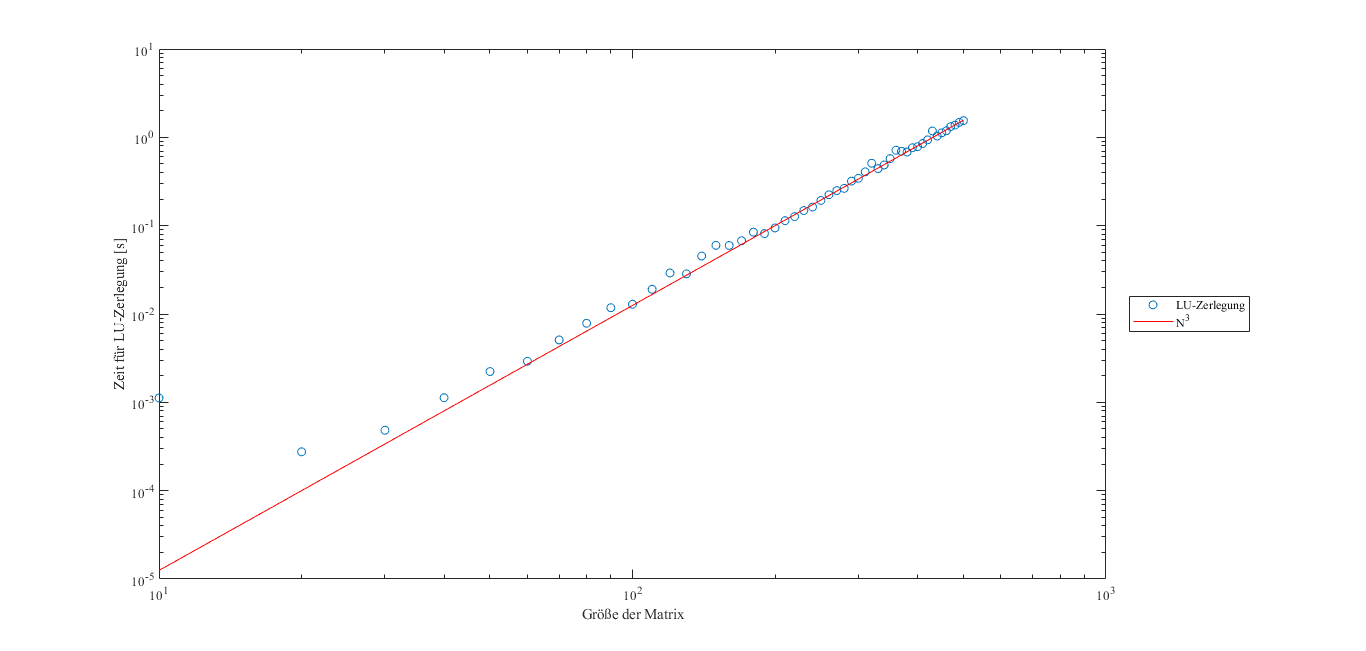
\includegraphics[scale=0.4]{Zeit10.png}
	\caption{Rechenzeit für die LU-Zerlegung einer $N\ \times\ N$-Matrix in Abhängigkeit der Matrixgröße $N$ im Vergleich zu einer Geraden mit Anstieg $N^3$} 
	\label{Abbildung1}
\end{figure}

Die in Abbildung \ref{Abbildung1} zu erkennende Kurve zeigt durch den Vergleich mit der Vergleichsgeraden $N^3$ und der logarithmischen Darstellung eindeutig ebenfalls einen solchen Anstieg für höhere N. Dieser Anstieg kommt zustanden, da die LU-Zerlegung durch eine dreifach ineinander verschachtelte Schleife implementiert wurde, wobei jeder dieser Schleifen $N$ Operationen durchführen muss. Bei Annahme eines linearen Zusammenhangs zwischen Rechenoperationen und Rechenzeit ergibt sich so ein Zusammenhang von $N^3$.
Der Grund für den schwächeren Zusammenhang für kleine N ist, dass in diesem Bereich die Rechenzeit viel mehr von z.B. Fluktuationen in der momentanen Leistung des Rechners  abhängt als bei höheren $N$. 

\end{document}